% !TeX root = ../thuthesis-example.tex

\chapter{Evaluation}\label{chapter-7}
In this section, we describe our efforts to evaluate the correctness and the performance of ExpertFlow. Evaluating the correctness amounts to ensuring that our system always produces the expected results, so that users can be confident that using ExpertFlow instead of another existing system will not result in obtaining wrong or low quality output tokens. Evaluating the performance allows us to check that ExpertFlow is faster or at least comparable to existing solutions.

\section{Evaluating correctness}\label{eval-correctness}
We evaluate the correctness of ExpertFlow through a combination of unit tests and integration-tests.

\subsection{Unit tests}
ExpertFlow inherits from FlexFlow~\cite{flexflow,unity}, the three levels of abstractions used to represent a DNN and execute its computations: \textit{layers}, \textit{operators}, and \textit{asynchronous tasks}, which in turn execute one (or more) \textit{kernel} on GPU. At each level of abstraction, we add multiple unit tests to verify the correctness under many different angles. For instance, at the layer level, we can most easily check the correctness of the structure of the model. At the operator level, we concentrate most tests that check the generated computational graph, the dimensions of the input and output tensors, and the parallelization strategies. At the task level, we can most easily check that the input and weights tensors are accessible, on the right device, and contain the correct data. Further, we can check the correctness of the GPU kernels. 

We implement our unit tests, organized as described above, using different programming languages and frameworks. At the layer, and operator level, we added tests in the form of assertions, based on quantities computed in C++, often based on the Legion library. We also used the DOT language, together with GraphViz, to export and visualize graph-structured quantities, such as the computational graphs, or the data and temporal dependencies between different tensors, operators, and tasks. Finally, we verified the correctness of all the custom kernels by re-implementing them using C++ and LibTorch (the PyTorch C++ API), running the CUDA and C++ versions in parallel, and verifying that the output tensors match. For the kernels that have a corresponding operator in PyTorch (e.g. the Linear layer, Softmax layer, LayerNorm, etc...), we also created a suite of \textit{alignment tests}, where we compare the output tensors of our kernels against the results obtained with PyTorch for a range of different input tensors. We added the alignment tests to CI, to ensure that we do not accidentally introduce new bugs with new commits.

\subsection{End-to-End tests}
After having tested each component individually, we used end-to-end tests as an additional check on the correctness of our implementation. We achieved this by choosing three representative models for which the pre-trained checkpoints is available, loading the weights into ExpertFlow, executing the same batch of inference requests using the original code and the ExpertFlow code representing the same model, and ensuring that the outputs match. In addition to loading the weights, we also needed to ensure that all the random seeds matched, whenever there was an operator with a stochastic behavior. The models we chose for this test were:
\begin{enumerate}
    \item LLAMA model~\cite{touvron2023llama} by Meta, a transformer model
    \item Fairseq’s 15B-parameters LM MoE model~\cite{fairseq-moe-model}, also by Meta, a MoE model
    \item GPT-MoE中文67亿诗歌生成模型~\cite{modelscope-checkpoint} by Modelscope, a MoE model
\end{enumerate}

\section{Evaluating performance}\label{eval-performance}
After evaluating the correctness of our framework, we ran several experiments to measure its performance. In the sections below, we discuss our experiment setup, and we present our results.

\subsection{Setup}
We run the experiments on a \texttt{g4dn.12xlarge} AWS machine with 48 vCPUs, 192 GiB of RAM memory, and 4 NVIDIA T4 GPUs (see Figure \ref{fig:gpu-setup}), each with 16 GB of memory (although the amount of usable memory is somewhat less). We initialize the instance with the Deep Learning AMI GPU PyTorch 1.13.0 (Ubuntu 20.04) 20221109. We run the FasterTransformer experiments within the \texttt{nvcr.io/nvidia/pytorch:22.07-py3} container, which comes with PyTorch built from source to add support for MPI, which is required by FasterTransformer to support the multi-GPU GPT program.

\begin{figure}[H]
    \centering
    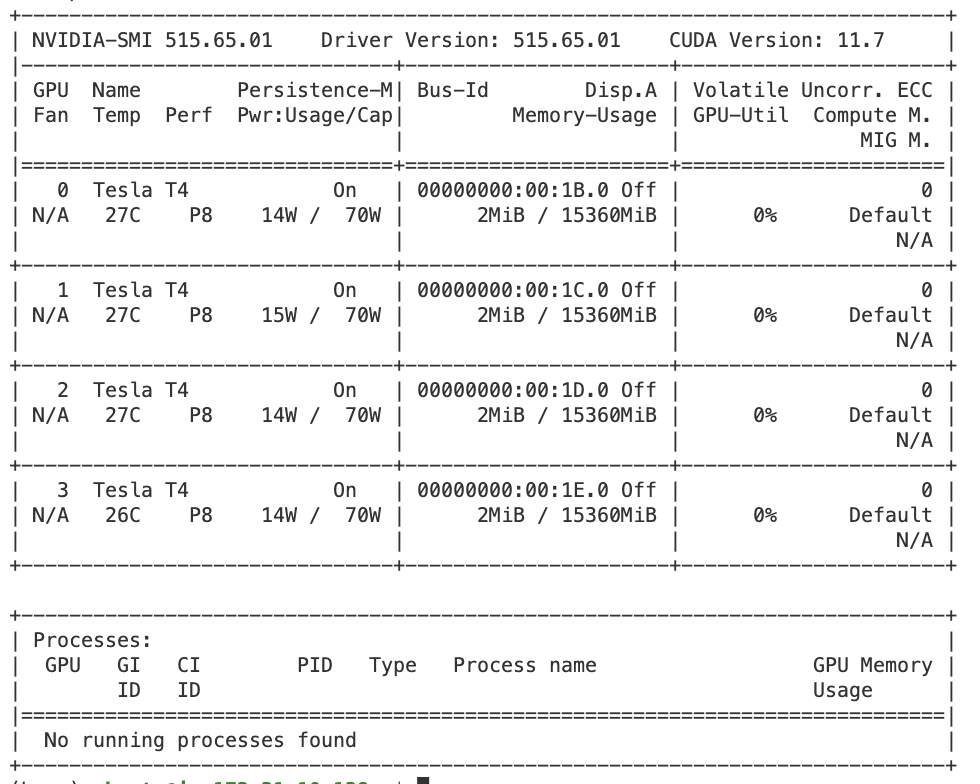
\includegraphics[width=\linewidth]{figures/nvidia-smi.png}
    \caption{\textbf{The GPU setup}}
    \label{fig:gpu-setup}
\end{figure}

\subsection{GPT-MoE model}
We ran our performance evaluation using the GPT-MoE model from Modelscope. We picked this model because it has full compatibility with FasterTransformer~\cite{faster_transformer}, as well as DeepSpeed~\cite{deepspeed-moe}, and the instructions for running it~\footnote{\url{https://github.com/NVIDIA/FasterTransformer/blob/main/docs/gpt\_guide.md\#gpt-with-moe}} in FasterTransformer are available in the GPT guide from the FasterTransformer Github repository. We use the provided scripts~\footnote{\url{https://github.com/NVIDIA/FasterTransformer/blob/main/examples/pytorch/gpt/utils/megatron\_gpt\_moe\_ckpt\_convert.py}} for converting the Modelscope checkpoint, which was built based on the Megatron-LM~\cite{megatron-lm} model specifications, to a format compatible with DeepSpeed and FasterTransformer. We then write our own custom scripts to convert and load the data into ExpertFlow.

The Modelscope MoE model is a fairly typical GPT-MoE model with 24 layers, half of which are regular FFN layers, and the other half are MoE. In particular, the odd-numbered layers are MoE. Regular FFN layers contain two dense layers, with an internal hidden dimension of size $4 \times$ as large as the hidden size. Each expert in the MoE layer also consists of two dense layers with an internal hidden dimension of size $4 \times$ as large as the hidden size. Additional settings are passed to the runtime via a human-readable \texttt{config.ini} file, whose contents are shown below (Listing \ref{config-ini}):

\begin{lstlisting}[language=Python, caption=config.ini, breaklines=true, basicstyle=\footnotesize, frame=single, label=config-ini]
[gpt]
model_name = gpt
head_num = 16
size_per_head = 64
inter_size = 4096
num_layer = 24
max_pos_seq_len = 2048
vocab_size = 51200
has_adapters = False
adapter_inter_size = 0
layernorm_eps = 1e-05
start_id = 50256
end_id = 50256
weight_data_type = fp16
tensor_para_size = 4

[structure]
gpt_with_moe = 1
expert_num = 64
moe_layers = [1, 3, 5, 7, 9, 11, 13, 15, 17, 19, 21, 23]
\end{lstlisting}


\subsection{Experiments}
\subsubsection{Workload generation}
The results of our experiments are shown below. We compare the performance of ExpertFlow to FasterTransformer, and report the throughput and latencies under different loads. We model the request arrivals using artificial traces where the arrival times are modeled by a Poisson process, and the request lengths follow a uniform distribution. This technique is similar to the approach taken in Orca~\cite{orca}. We build a workload generator that takes as input the following parameters:
\begin{itemize}
    \item the average requet arrival rate ($\lambda$)
    \item the total number of requests ($N$)
    \item the minimum ($p_{min}$) and maximum length ($p_{max}$) of the prompt
    \item the minimum ($g_{min}$) and maximum number ($g_{max}$) of tokens to generate
\end{itemize}
Given the values of the parameters above, our generator works as follows. For each request $k$, it generate the request's arrival time ($t_k$) by sampling from the Erlang distribution:
\begin{equation}
    T=\{t_1,..., T_N\} \sim Erlang(k, \lambda)
\end{equation}
The PDF of the Erlang distribution is as follows: 
\begin{equation}
    p_{T_k} = P(T_k=t)=\frac{\lambda^kt^{k-1}e^{-\lambda t}}{(k-1)!}
\end{equation}
From an implementation standpoint, we can simulate each request arrival time $t_k$, using just a uniform random number generator and the following formula: 
\begin{equation}
    t_k=-(1/k)\sum_{i=1}^k\log{u_i}
\end{equation}
where $u_i$ is the $i$-th random number generated from the uniform distribution 
\begin{equation}
    U \sim Uniform([0,1])
\end{equation}
Next, the number of tokens in the prompt $p_k$ and the number of tokens to generate ($g_k$) as output in each request are determined by sampling from the following uniform distributions:
\begin{align}
    p_k & \sim Uniform([p_{min}, p_{max}]) \\
    g_k & \sim Uniform([g_{min}, g_{max}])
\end{align}
Given the value of $p_k$, we generate the request's prompt by randomly sampling $p_k$ values from the range of integers $[0, vocab\_size -1]$.
In summary, each request $k \in [0, N-1]$ is generated using the three parameters $t_k$ (arrival time), $p_k$ (\# input tokens) and $g_k$ (\# output tokens). 
\subsubsection{End-to-End Results}
Below, we provide the results for 4 different workloads, with $\lambda = 50, 100, 250, 500$ requests/second, $N = 2560$, $p_{min} = 8$, $p_{max} = 128$, $g_{min} = 1 $, $g_{max} = 256 - p_{max}$. Table \ref{tab:req-throughput} shows the throughput (in terms of requests processed per second) for the arrival rates mentioned above. Table \ref{tab:token-throughput} shows the throughput (in terms of tokens processed per second) for the arrival rates mentioned above. We provide two different measurements for the throughput because the requests have different lengths, so it is not possible to simply calculate the tokens/s throughput from the request/s throughput. Next, Table \ref{tab:conv-perf-detail} presents the statistics regarding the latency.

\begin{table}[H]
\caption{Request serving throughput (requests/s) }
%\vspace{-1em}
\label{tab:req-throughput}
\resizebox{\linewidth}{!}{
\centering
\begin{tabular}{c|c|c}
\toprule
Arrival rate (requests/s) & ExpertFlow throughput (requests/s) & FasterTransformer throughput (requests/s) \\
\midrule
50 & 48.302 & - \\
100 & 83.190 & 53.736 \\
250 & 105.239 & 54.399 \\
500 & 105.524 & 54.226 \\
\bottomrule
\end{tabular}
}
\end{table}

\begin{table}[H]
\caption{Token generation throughput (token/s) }
%\vspace{-1em}
\label{tab:token-throughput}
\resizebox{\linewidth}{!}{
\centering
\begin{tabular}{c|c|c}
\toprule
Arrival rate (requests/s) & ExpertFlow throughput (tokens/s) & FasterTransformer throughput (tokens/s) \\
\midrule
50 & 3119.0 & - \\
100 & 5373.75 & 3471.18 \\
250 & 6806.7 & 3518.42 \\
500 & 6815.65 & 3502.37 \\
\bottomrule
\end{tabular}
}
\end{table}

\begin{table}[H]
\caption{Inference latency per request}
\label{tab:conv-perf-detail}
%\scriptsize
\centering
\begin{tabular}{c|c|cccc}
\toprule
  Arrival rate (requests/s)  & Inference System & \textbf{Average (ms)}  & \textbf{Min (ms)} & \textbf{Max (ms)} \\
\midrule
\multirow{2}{*}{50} & ExpertFlow & 8,475.191 & 5,621.950 & 12,886.612 \\
                    & FasterTransformer & - & - &  -   \\
\midrule
\multirow{2}{*}{100}  & ExpertFlow & 10,217.809 & 5,674.259 & 17,971.726  \\
 & FasterTransformer & 10,747.242   & 277.899 & 21,115.594  \\
\midrule
\multirow{2}{*}{250}  & ExpertFlow & 16,223.166 & 5,862.399 & 25,789.413  \\
 & FasterTransformer & 18,646.640   & 224.331 & 36,858.986  \\
\midrule
\multirow{2}{*}{500}  & ExpertFlow & 18,541.337 & 6,141.7325 & 25,671.801  \\
 & FasterTransformer & 21,297.635   & 275.063 & 42,134.64  \\
\bottomrule
\end{tabular}
\end{table}

Note that in the tables above, the results from FasterTransformer are missing for $\lambda=50$ requests/s due to an issue with the framework, such that the execution of the MoE example from FasterTransformer hangs forever when the arrival rate is too low. We are currently working on fixing this bug.

Finally, we plot the latency as a function of the request length. We can see that curve from FasterTransformer is much more noisy than the one from ExpertFlow, and there seems to be a weaker correlation between between the latency and the request length. This is likely due to the padding required when batches of requests have different lengths. 

\begin{figure}[H]
    \centering
    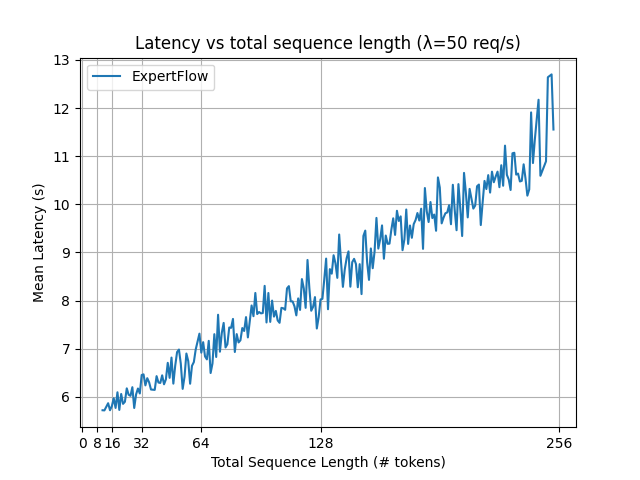
\includegraphics[width=0.6\linewidth]{figures/rate50.png}
    \caption{\textbf{The latency of serving a request as a function of the final request length} ($\lambda=50$ requests/second)}
    \label{fig:rate50}
\end{figure}

\begin{figure}[H]
    \centering
    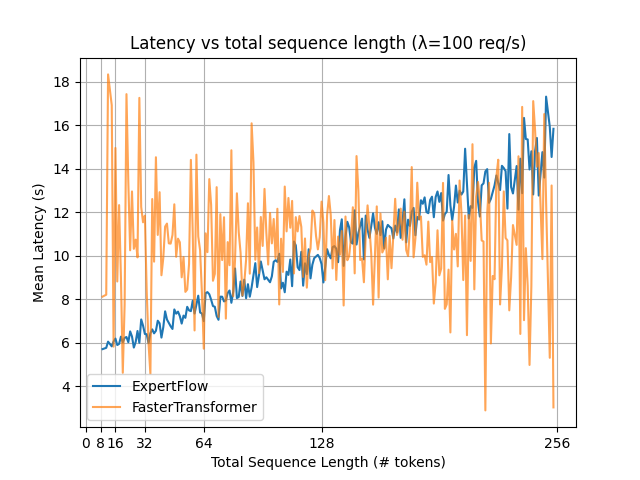
\includegraphics[width=0.6\linewidth]{figures/rate100.png}
    \caption{\textbf{The latency of serving a request as a function of the final request length} ($\lambda=100$ requests/second)}
    \label{fig:rate100}
\end{figure}

\begin{figure}[H]
    \centering
    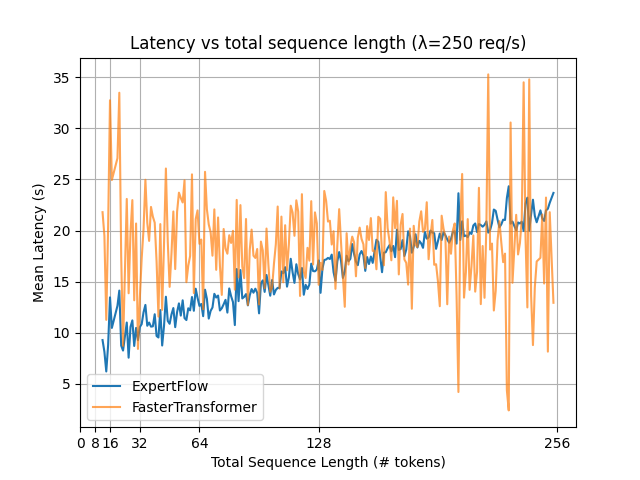
\includegraphics[width=0.6\linewidth]{figures/rate250.png}
    \caption{\textbf{The latency of serving a request as a function of the final request length} ($\lambda=250$ requests/second)}
    \label{fig:rate250}
\end{figure}

\begin{figure}[H]
    \centering
    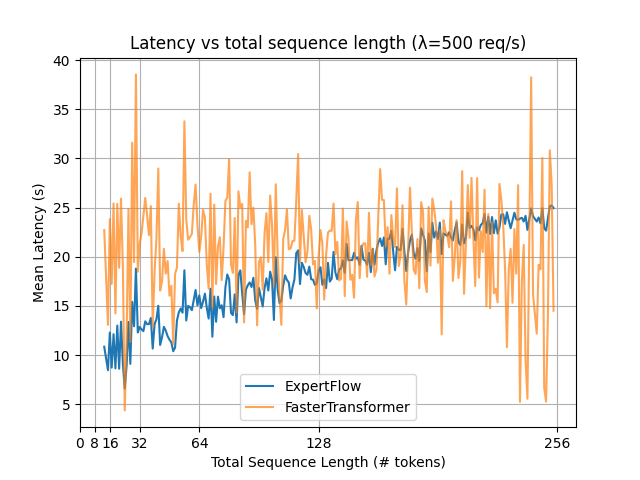
\includegraphics[width=0.6\linewidth]{figures/rate500.png}
    \caption{\textbf{The latency of serving a request as a function of the final request length} ($\lambda=500$ requests/second)}
    \label{fig:rate500}
\end{figure}

\subsubsection{Speculative Inference Evaluation}
We evaluate the performance of speculative inference by measuring the speedup compared to incremental decoding. We use 5 publicly-available prompt datasets, and first run the LLAMA-7B model in incremental decoding mode, measuring the execution time. Next, we repeat the experiment and use the LLAMA-7B model for token-tree verification, and use a set of speculators derived from LLAMA-160M. We observe speedups between 1.91x and 2.75x, as shown in Figure \ref{fig:latency}.

\begin{figure}
    \centering
    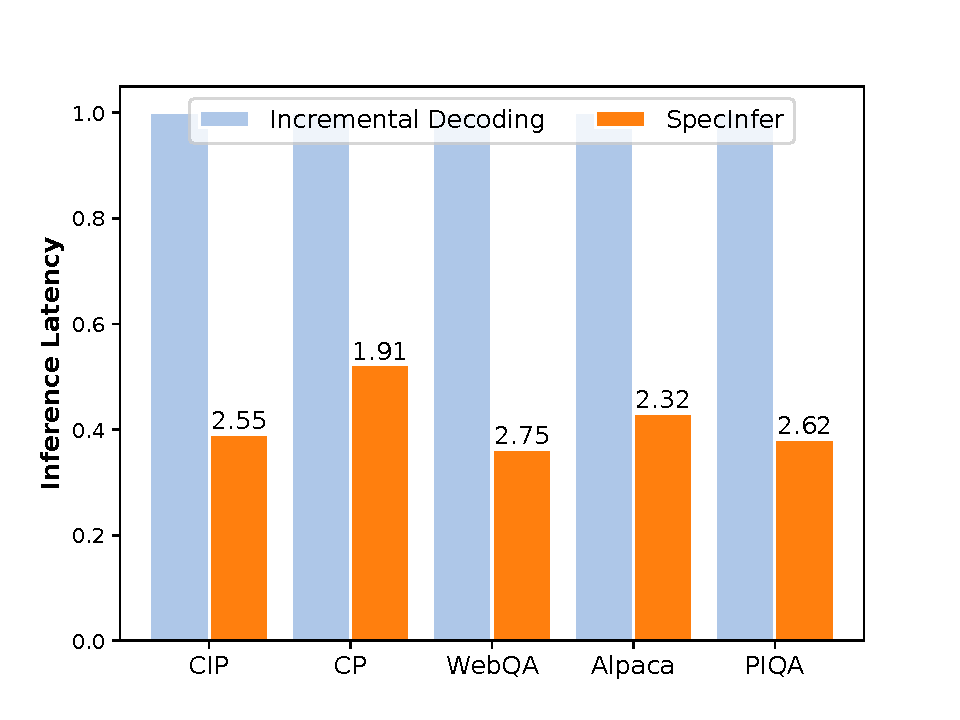
\includegraphics[scale=0.45]{figures/latency_improvement.pdf}
    \caption{\textbf{End-to-end inference latency speedup of speculative inference} when compared to incremental decoding, using five public prompt datasets. We use LLAMA-7B as the LLM and all SSMs are derived from LLAMA-160M}
    \label{fig:latency}
\end{figure}

\subsubsection{Future work}
Additional experiments could be useful to better understand the performance of ExpertFlow, the bottlenecks, and potential avenues for further improvement. Due to time constraints, we did not include these experiments in the current version of this document. Hence, we leave them to future work. Possible directions for additional evaluation efforts could be: an ablation study to evaluate the contribution of each of the system components towards the end-to-end performance; comparing our throughput and latency to DeepSpeed-MoE; running experiments under different sets of configurations. 

\section{Conclusion}
In this chapter, we described our efforts to evaluate the correctness and performance of ExpertFlow. In Section \ref{eval-correctness} we illustrated how we used unit and integration tests to ensure that our system can produce correct results, which align with other inference systems. In Section \ref{eval-performance}, we explained the setup for our experiments, and provided the results to measure the performance of ExpertFlow when compared to the baseline.